\begin{savequote}[6cm]
<< Is this thing on? I don't think this thing is on. Hello! [...] Confangled modern doohickeys. >>
\qauthor{Grany Smith}
\end{savequote}

\chapter{Astronef : De l'expression à l'exécution}\label{chap:contrib:astronef}
\chaptertoc

Astral est une algèbre permettant d'exécuter des requêtes continues sans ambiguïtés sémantiques. Les concepts développés au chapitre~\ref{chap:contrib:astral} ne sont pas attachés à un mode d'exécution ou à une implémentation particulière. Dans ce chapitre, nous présentons l'intergiciel \textit{Astronef}\footnote{Astral Optimization and Execution Framework} permettant l'exécution de requêtes continues Astral. Dans cette mise en œuvre, nous focalisons notre attention sur trois points en particulier :
\begin{itemize}
	\item[\textbf{Conformité à Astral}] : Nous avons développé un modèle expressif et libre de toute ambiguïté. Il est important que les composants développés dans cette mise en œuvre correspondent aux sémantiques qu'ils sont capables d'exécuter en Astral.
	\item[\textbf{Extensibilité}] : L'utilisateur doit pouvoir adapter l'intergiciel à son utilisation. Ainsi, il doit pouvoir ajouter ou reconfigurer des composants à la volée.
	\item[\textbf{Optimisation}] : L'intergiciel doit être capable de fournir un plan d'exécution efficace pour une requête donnée.
\end{itemize}

La section~\ref{sec:contrib:astronef:architecture} présente l'architecture générale d'Astronef. La section~\ref{sec:contrib:astronef:preparation} présente notre approche à base de règle pour construire un plan de requête. La section~\ref{sec:contrib:astronef:logique} présente la première partie de l'optimisation du plan : l'optimisation logique, permettant de réécrire une requête de manière plus efficace. Puis nous détaillons en section~\ref{sec:contrib:astronef:physique} la seconde partie de l'optimisation : l'optimisation physique permettant de sélectionner les meilleurs composants pour exécuter le plan de requête. Enfin, nous analysons en section~\ref{sec:contrib:astronef:integration} les impacts de l'intégration d'un nouveau composant à l'architecture. Nous concluons ce chapitre en section~\ref{sec:contrib:astronef:conclusion}.

\lstset{language=PrologAstral}
\section{Architecture interne d'Astronef}\label{sec:contrib:astronef:architecture}
Dans cette section, nous détaillons les éléments d'architecture que nous avons mis en œuvre pour permettre à une requête Astral d'être instanciée en un processus de traitement. Nous abordons premièrement les principes architecturaux utilisés. Ensuite, nous détaillons les différents composants utilisés dans Astronef. Enfin, nous présentons notre méthode extensible de construction de plan par l'utilisation d'un système de règles.
\subsection{Choix d'architecture logicielle}
Avant de détailler l'architecture de notre système de traitement de requêtes continues, nous allons d'abord présenter le paradigme architectural dans lequel nous allons mettre en œuvre Astronef. Nous présentons premièrement et brièvement les architectures à services. Puis, nous détaillons les principes des architectures à composants orientés services que nous utilisons par la suite.
\subsubsection{Architecture à service}
Les architectures à services permettent aux applications d'être assemblés sous forme de blocs réutilisables : des \textit{services}. Un \textit{service} est définit par une spécification (ou \textit{description}, ou \textit{contrat}), qui décrit sa syntaxe, son comportement, sa sémantique ainsi que sa dépendance aux autres services. Dans les architectures à services, les services interagissent via un patron récurrent d'interaction (fig~\ref{fig:contrib:astronef:services}). 
\begin{figure}[ht]
    \centering
    \includegraphics[width=0.7\textwidth]{contrib-astronef-services}
    \caption{Patron d'interaction de service}\label{fig:contrib:astronef:services}
\end{figure}
Un fournisseur de service va publier sa spécification à un registre. Un consommateur de service découvre le service fournit par une requête sur le registre. Enfin, le consommateur et le fournisseur se connectent. Le point clé est que la résolution est faite à l'exécution.

\subsubsection{Architecture à composants orientés services}
Le modèle d'architecture à composants orientés services~\cite{Cervantes:servicecomponent} permet la mise en œuvre d'applications à base de services dans le paradigme de la programmation par composants. Le principe est de séparer les mécanismes des architectures à services du code implémentant le comportement du service fournit. Ainsi, les principes d'un tel modèle sont :
\begin{itemize}
    \item Un service est une fonctionnalité fournie.
    \item Un service est caractérisé par sa spécification.
    \item Les composants implémentent des spécifications de services, qui peuvent eux-mêmes dépendre, du fait de leurs implémentations, d'autres services.
    \item Les patrons d'interactions de services sont utilisés pour résoudre les dépendances de services à l'exécution.
    \item Les compositions sont décrites en terme de spécifications de services.
    \item Tout composant peut se substituer par un autre si les spécifications de services sont identiques.
\end{itemize}
Le modèle combine les idées de composants et de services. De plus, en s'inspirant des modèles tels que Fractal~\cite{Bruneton:fractal}, chaque composant possède un ensemble de propriétés (ou attributs) configurables. Nous obtenons aussi le pouvoir d'instancier (grâce aux fabriques) des composants à partir de configurations.

\begin{figure}[ht]
    \centering
    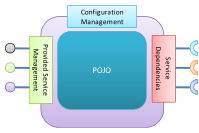
\includegraphics[width=0.5\textwidth]{contrib-astronef-ipojo}
    \caption{Un composant iPojo}\label{fig:contrib:astronef:ipojo}
\end{figure}
La figure~\ref{fig:contrib:astronef:ipojo} représente un composant dans l'implémentation \textit{iPojo}~\cite{Escoffier:ipojo}. Le code du composant (le \textit{POJO}, \textit{Plain Old Java Object}) est embarqué dans un conteneur auxquels sont accrochés des gestionnaires. Les trois couramment utilisés sont les gestionnaires de dépendances, de production de service, et de configuration. Ainsi, un composant peut s'exposer sur un registre, tout en dépendant d'autres services et en étant configurable.

\subsection{Les composants et services d'Astronef}
L'architecture d'Astronef est entièrement dirigé par les approches de composants orientés services. De multiples composants sont créés et instantiés, pour former une requête. Afin de pouvoir exécuter les requêtes, nous définissons trois services centraux :
\begin{itemize}
	\item[\textbf{Les services \textit{EventProcessor}}] ont deux primitives, l'une exécute une tâche, l'autre indique les \textit{EventProcessors} devant être exécutés avant soi-même.
	\item[\textbf{Le service \textit{Scheduler}}] permet la planification. Ses primitives permettent aux différents \textit{EventProcessor} d'exprimer leur volonté de s'exécuter. Ce service établit l'ordonnancement de ces demandes en fonction des contraintes des \textit{EventProcessor}s.
	\item[\textbf{Le service \textit{QueryRuntime}}] permet d'exécuter une requête. Il est lié à un \textit{Scheduler} et utilise la primitive \textit{next} de celui-ci pour connaître la prochaine tâche à exécuter.
\end{itemize}

Nous adoptons l'approche émise par~\cite{Carney:scheduling} en gérant l'ordonnancement par un service externes aux opérateurs, comme présenté dans la section~\ref{sec:rw:sgfd:infra}. Maintenant que nous avons vu les différents services nécessaire à l'exécution. Nous avons plusieurs types de composants que nous pouvons instantier par des services de fabriques :
\begin{itemize}
	\item[\textbf{Les flux ou relations} (entités)] : Fournissent les primitives nécessaires à leur manipulation par Astral. Ces entités servent de résultats intermédiaires (ou de tampons). De plus, ils permettent un service de notification. En cas de changement, les \textit{EventProcessor} abonnés sont notifiés. Ainsi, ces composants nécessitent un \textit{Scheduler} pour demander l'exécution de leurs abonnés.
	\item[\textbf{Les sources}] : Une source nécessite une entité qu'elle alimente grâce aux données issues d'origines diverses (protocoles réseaux, fichiers,...). Ce composant peut nécessiter le \textit{Scheduler} pour, entre autres, notifier sa fin de vie ce qui peut engendrer la fin de vie de la requête.
	\item[\textbf{Les opérateurs}] : Nécessitent $n$ entités en lecture, et une autre particulière en écriture. Ce composant doit fournir le service \textit{EventProcessor}. Les implémentations des opérateurs bloquants peuvent faire appel au \textit{Scheduler} pour planifier des exécutions ponctuelles.
	\item[\textbf{Les puits}] : Nécessitent une entité en lecture. Ce composant fournit le service \textit{EventProcessor} et doit être non-bloquant.
\end{itemize}

Ainsi pour créer une requête : l'utilisateur de l'intergiciel doit fournir un ou plusieurs composants sources et un composant puit. Par la suite, il demande à Astronef de lui instantier ses sources et son puit en configurant les composants selon sa volonté. Enfin, il spécifie l'expression algébrique liant les sources au puit.

\subsubsection{De l'importance de la réutilisation}
\textit{Astronef} permet une grande flexibilité grâce aux composants orientés services. Tout d'abord, chaque composant peut être configuré tout en gérant son cycle de vie, ce qui permet de réutiliser le même module pour plusieurs usages. Par exemple, supposons l'existence d'une source capable de récupérer une information périodiquement sur un dispositif $D$ via un protocole donné. Cette source peut être utilisée pour plusieurs requêtes sous différentes instances en ayant plusieurs configurations : différents dispositifs ou périodes d'acquisitions.

Cette abstraction sous forme de services permet surtout la substitution. En effet, nous pouvons remplacer tout composant par un autre supportant le même service. Nous utilisons ce principe pour sélectionner les meilleurs composants pour remplir le plus efficacement leurs rôles. De plus, l'utilisateur peut apporter ses propres implémentations pour étendre les capacités de l'intergiciel.

\section{De l'algèbre aux composants}\label{sec:contrib:astronef:preparation}
A tout composant est attaché une fabrique permettant de créer les instances. Pour construire une requête, l'utilisateur peut faire appel à chaque fabrique pour instancier chaque source, opérateurs, entités, et puits. Une fois les composants construit et liés entre eux, il peut demander au moteur de créer un service \textit{QueryRuntime} pour exécuter la requête. Toutefois, nous souhaitons pouvoir exploiter les connaissances d'Astral pour aider à la construction de ce plan d'exécution.

Nous souhaitons que l'utilisateur n'ait pas à intervenir lors de cette construction. De son point de vue, il ne doit écrire que l'expression algébrique de sa requête et il doit être garanti d'une mise en œuvre efficace. Cette section détaille notre approche. Tout d'abord, nous détaillons l'idée de la construction du plan d'exécution par règles. Ensuite, nous présentons les choix technologiques mis en œuvres. Enfin, nous voyons comment préparer la requête à l'optimisation que nous détaillons dans les sections suivantes.

\subsection{Approche de la construction par inférence}
Pour atteindre ce but, nous avons choisi de mettre en place une approche à base de règle. En partant de l'expression algébrique, nous itérons suivant plusieurs règles d'inférence jusqu'à l'obtention d'un plan de requête. Nous remarquons plusieurs avantage à une telle approche :
\begin{itemize}
	\item Intégration naturelle des connaissances. Les propriétés de l'algèbre peuvent s'exprimer dans un langage déclaratif pour les exploiter.
	\item Expression de la sémantique des composants par l'algèbre. Comme il est nécessaire d'associer la sémantique d'Astral aux composants logiciels, il est nécessaire de spécifier à quelle opération chaque composant (et chaque paramètre de configuration) répond. Cela permet une clarification des sémantiques d'exécution.
	\item Extensibilité très forte. En considérant que l'ajout de nouveaux composants peut se faire via l'ajout de nouvelles règles, il devient aisé d'étendre le système pour permettre des opérateurs, ou des optimisations qui n'étaient pas prévues.
\end{itemize}

\subsubsection{Optimisation par heuristiques}
Afin de mettre en œuvre cet ensemble de règle pour obtenir un plan de requête efficace, nous introduisons une optimisation logique et physique à l'image des optimisations des SGBD. Nous restructurons la structure de l'expression algébrique dans la section~\ref{sec:contrib:astronef:logique} pour qu'elle soit plus optimisé. Ensuite, nous sélectionnons les meilleurs composants et les meilleures configurations pour mettre en œuvre cette nouvelle expression, dans la section~\ref{sec:contrib:astronef:physique}.

Toutefois, dans notre contexte, nous ne pouvons pas appliquer directement certaines optimisations des SGBDs. Contrairement aux règles habituelles, nous ne réordonnons pas les jointures du fait du théorème~\ref{thm:asymetrie}. De plus, la notion d'entrée-sortie est réduite à une notion de résultats intermédiaires, même au niveau des sources (rendant l'utilisation des index moins pertinent que sur disque). En effet, la performance se mesure généralement en débit supporté et les débits de sources sont a priori inconnus. Au total, un gain de performance est mesuré sur un gain de consommation processeur et, à moindre mesure, sur une consommation mémoire contrôlée (ou bornée).

De plus, Astral possède plus d'opérateurs et de restrictions que l'algèbre relationnelle ce qui rend l'espace de recherche plus large. Ainsi, nous développons plusieurs heuristiques nous permettant de faire les différentes réécritures par applications de règles.

\begin{figure}[ht]
	\centering
	\includegraphics[width=0.9\textwidth]{contrib-astronef-optimisation}
	\caption{Processus d'optimisation d'une requête algébrique dans Astronef}\label{fig:contrib:astronef:optimisation}
\end{figure}
La figure~\ref{fig:contrib:astronef:optimisation} représente le processus total d'optimisation d'une requête algébrique. Nous pouvons clairement distinguer trois parties, la phase de préparation, puis l'optimisation logique et enfin physique. Chaque sous-tâche est détaillé dans les sections suivante.

\subsection{Choix technologiques}
Nous utilisons un moteur capable d'exécuter du Prolog~\footnote{En réalité, le langage utilisé (PROVA~\cite{Kozlenkov:prova}) est un dérivé de Prolog mieux adapté à l'intégration avec Java. Mais le principe reste similaire.}, langage de programmation logique, pour appliquer nos règles. Avant de détailler l'ensemble de ces règles, nous présentons d'abord la structure d'une expression. Toute expression est structurée sous forme d'arbre, il est possible de représenter une requête avec des nœuds de la forme\footnote{L'utilisation d'objets de propriétés fait partie du langage PROVA, mais cela reste formalisable en Prolog standard avec une liste d'éléments [clé,valeur].} :
\begin{center} [$\underbrace{A}_{\textrm{Nature du nœud}}$, $\underbrace{B}_{\textrm{Ensemble de propriétés}}$, $\underbrace{C}_{\textrm{Liste de nœuds fils}}$] \end{center}
\begin{example}
	Soit $R$ une source déclaré dans le système, nous souhaitons exécuter la requête $\sigma_{id=1} R$. L'expression de cette requête en PROVA est la suivante :
	\begin{lstlisting}
[sigma,	{"condition":"id=1"}, [
	[source, {id:"R"}, []]
]]
	\end{lstlisting}
\end{example}
Nous remarquons que cette syntaxe est très similaire au \textit{XML} : chaque nœud possède un nom, un ensemble de propriétés et un ensemble de fils, tout comme les balises \textit{XML}. C'est pour cela que ce langage est celui utilisé en pratique pour spécifier des requêtes dans le prototype. Il est ensuite traduit en expression utilisable en Prolog. L'ensemble des nœuds possibles corresponds aux différents opérateurs de l'algèbre. Nous ne détaillons pas cet aspect dans ce manuscrit. Le lecteur peut consulter le manuel sur la page web suivante \url{http://code.google.com/p/astral/wiki/XMLSyntax} pour trouver les expressions exactes supportées.


\subsection{Préparation de la requête}
Afin de pouvoir commencer à raisonner sur l'expression algébrique, nous devons tout d'abord préparer l'arbre de requête. Nous présentons l'ensemble de la phase de préparation composé du remplacement des sucres syntaxiques, de l'inférence des types et de l'inférences des attributs des résultats intermédiaires.
\subsubsection{Sucres syntaxiques}
Un sucre syntaxique permet d'aider l'utilisateur à écrire et lire son expression algébrique. Afin de pouvoir appliquer des règles sur l'arbre de requête, nous devons remplacer ces sucres syntaxiques par leurs expressions en termes d'opérateurs primitifs Astral. Par exemple, l'opérateur $\ssjoin$ est une composition d'opérateur $\Join$ et $\D_f^c$, l'opérateur $[L]$ correspond à l'opérateur $[j,j,1]$.

\begin{regle}[Sucres syntaxiques]
Le remplacement des sucres syntaxiques transformant l'expression $[A1,B1,C1]$ en $[A2,B2,C2]$ se fait par le prédicat :
\begin{center} \textbf{sugar}($[A1,B1,C1]$, $[A2,B2,C2]$).\end{center}
Ce prédicat est appliqué tant qu'il peut l'être (de manière itérative).
\end{regle}

\begin{example}
	Nous nous proposons de remplacer le sucre syntaxique $R^{t_0}$ en $\D^{t0} (R)$. $R^{t_0}$ est exprimée par le nœud \textit{freeze} possédant le paramètre \enquote{at} et $\D$ est exprimée par un nœud \textit{timetransform} possédant un paramètre \enquote{description}. Voici l'expression de ce remplacement :
	\begin{lstlisting}
sugar(
	[freeze, % Lorsqu'il existe un noeud freeze
		{at: t0},
		Children], 
	[timetransform, % ... le remplacer par timetransform
		{"description": [ % Avec un parametre description
		% contenant le type de manipulation voulue
			{"type": "freeze", 
			"at": t0}
		]},
		Children]
).
	\end{lstlisting}
\end{example}

Ce prédicat est de plus utilisé pour analyser les chaînes de caractères ce qui permet, par exemple, d'extraire la liste des attributs de conditions ou d'expressions.

\subsubsection{Inférences des types et attributs}
Afin de pouvoir traiter correctement les différents nœuds, il nous faut inférer les deux propriétés majeures de chaque nœud d'une requête qui va définir la nature de son résultat intermédiaire : son type (\textit{flux} ou \textit{relation}) et ses attributs. Pour cela, il faut être garanti que les sources exposent leurs attributs et types dans leurs propriétés. Par la suite, un programme applique ces règles de façon récursive. Les résultats sont stockés dans les propriétés \textit{type} et \textit{attributes}.

\begin{regle}[Inférences des types]
L'inférence du type $Type$ de l'expression $[A,B,C]$ dont les types fils sont $TypesFils=[T1,...]$ se fait par le prédicat :
\begin{center} \textbf{typerules}($[A,B,C,TypesFils]$, $Type$).\end{center}
Ce prédicat s'applique de manière récursive.
\end{regle}

\begin{regle}[Inférences des attributs]
L'inférence de la liste d'attributs d'un nœud $[A,B,C]$ dont les attributs fils sont $AttributsFils$ se fait par le prédicat :
\begin{center} \textbf{attribrules}($[A,B,C,AttributsFils]$, $Attributs$).\end{center}
Ce prédicat s'applique de manière récursive.
\end{regle}

\begin{example}
	Pour la définition de la jointure dans Astronef, les règles sont simples. La liste des attributs est l'union des listes d'attributs fils. Et le type de la jointure est relationnel si ses fils le sont aussi.
	\begin{lstlisting}
typerules([join,_,_, TypesFils], Type):- 
	allequal(TypesFils,Type), % Verification que tous soient relationnels 
	relation(Type), !.
attribrules([join,_,_,AttributsFils], Attributs):- !, 
	union(AttributsFils,Attributs).
	\end{lstlisting}
\end{example}

Voyons désormais un exemple simple sur la jointure de deux relations.
\begin{example}
	Soit la requête $S[B] \Join_{a < b} R$. Son expression correspondante en Prolog est :
	\begin{lstlisting}
[join, {condition: "a < b"}, [
	[window, {description: [{type: "B"}]}, [
		[source, {id: "S", attributes: ["a", "T"], type: "stream"}, []]
	]],
	[source, {id: "R", attributes=["b", "c", "d"], type: "relation"}, []]
]]
	\end{lstlisting}
	Après la phase de préparation, nous obtenons l'expression suivante :
	\begin{lstlisting}
[join, {condition: "a < b", conditionAttributes: ["a", "b"], 
		 type: "relation", attributes: ["a", "b", "c", "d", "T"]}, [
	[window, {description: [{type: "B"}], 
			   type: "relation", attributes: ["a", "T"]}, [
		[source, {id: "S", attributes: ["a", "T"], type: "stream"}, []]
	]],
	[source, {id: "R", attributes=["b", "c", "d"], type: "relation"}, []]
]]
	\end{lstlisting}
	Nous remarquons que les propriétés \textit{type} et \textit{attributes} existent sur tous les nœuds maintenant. De plus, la propriété \textit{conditionAttributes} a été placée sur la jointure.
\end{example}
Après le remplacement des sucres syntaxiques et l'inférence des types et attributes, l'évaluation procède à l'optimisation logique.
\section{Optimisation logique}\label{sec:contrib:astronef:logique}
Cette première application de règles permet de restructurer l'expression de la requête pour avoir la structure la plus adéquate. Dans cette section, nous pourrons exploiter les connaissances accumulés dans les théorèmes d'Astral que nous pourrons retrouver dans le chapitre~\ref{chap:validation:expressivite}.
\subsection{Préparation}
Tout d'abord, il est nécessaire d'appliquer les sucres syntaxiques pouvant être présents dans l'expression. Par exemple, l'opérateur $\ssjoin$ est un opérateur composite qui n'est défini que par la composition d'autres opérateurs primitifs.

\begin{regle}[Sucres syntaxiques]
L'application de sucre syntaxique transformant l'expression $[A1,B1,C1]$ en $[A2,B2,C2]$ se fait par le prédicat :
\begin{center} \textbf{sugar}($[A1,B1,C1]$, $[A2,B2,C2]$).\end{center}
Ce prédicat est appliqué tant qu'il peut l'être (de manière itérative).
\end{regle}

\begin{example}
	Nous nous proposons d'appliquer le sucre syntaxique pour transformer $\Join_c$ en $\sigma_c \Join$. Pour rappel, le prédicat \textit{sugar} sera appliqué si et seulement si ses conditions sont vérifiées. Ici, nous vérifions qu'il y a une condition \textit{Cond} dans les propriétés. Par la suite, nous pouvons transformer la jointure en sélection-jointure (après avoir retiré la condition des propriétés évidemment).
	\begin{lstlisting}
sugar(
	[join,B,C], 
	[sigma, {"condition": Cond}, [
		[join,BOut,C]
	]]
):-
    	map_get(B, "condition", Cond), %La jointure est avec condition
    	!, % alors...
    	map_remove(B, "condition", BOut). %Suppression de la condition
	\end{lstlisting}
\end{example}

Maintenant, afin de pouvoir traiter correctement les différents nœuds, il nous faut inférer les deux propriétés majeures de chaque nœud d'une requête qui va définir la nature de son résultat intermédiaire : son type (\textit{flux} ou \textit{relation}) et ses attributs. Pour cela, il faut être garanti que les sources exposent leurs attributs et types dans leurs propriétés. Par la suite, un programme appliquera ces règles de façon récursive. Les résultats seront stockés dans les propriétés \textit{type} et \textit{attributes}.

\begin{regle}[Inférences de types et d'attributs]
L'inférence du type $Type$ de l'expression $[A,B,C]$ dont les types fils sont $TypesFils=[T1,...]$ se fait par le prédicat :
\begin{center} \textbf{typerules}($[A,B,C,TypesFils]$, $Type$).\end{center}
De façon similaire, nous obtenons pour la liste d'attributs d'un nœud :
\begin{center} \textbf{attribrules}($[A,B,C,AttributsFils]$, $Attributs$).\end{center}
Ceux deux prédicats s'appliquent de manière récursive, d'abord la projection puis la sélection.
\end{regle}


\begin{example}
	Pour la définition de la jointure, les règles sont simples. Le liste des attributs est l'union des listes d'attributs fils. Et le type est du relationnel vers le relationnel.
	\begin{lstlisting}
typerules([join,_,_, TypesFils], Type):- 
	allequal(TypesFils,Type), % Verification que tous soient relationnels 
	relation(Type), !.
attribrules([join,_,_,AttributsFils], Attributs):- !, 
	union(AttributsFils,Attributs).
	\end{lstlisting}
\end{example}

Nous avons maintenant un arbre prêt à être optimisé. Tout d'abord, appliquons les règles les plus classiques dans l'optimisation de requêtes en gestion de base de données : la projection.

\subsection{Projection et sélection}
Cette optimisation permet de réduire l'empreinte mémoire des résultats intermédiaires ce qui de plus réduira les temps de calculs des opérateurs. Pour atteindre ce résultat, il est nécessaire d'appliquer les résultats que nous donne Astral. Ces résultats seront tous présentés dans le chapitre~\ref{chap:validation:expressivite}. Nous pouvons tout de même présenter le prédicat logique qui devra appliquer ces règles.
\begin{regle}[Pousser les projections et sélections]
La transformation d'un nœud contenant la projection afin de l'appliquer sur ses nœuds fils est gérée par le prédicat suivant :
\begin{center} \textbf{pushprojectionrule}($[pi,BPi,[[A,B,C]]],[AOut,BOut,COut]$).\end{center}
De façon similaire, la sélection est gérée par le prédicat :
\begin{center} \textbf{pushselectionrule}($[sigma,BSigma,[[A,B,C]]],[AOut,BOut,COut]$).\end{center}
Ceux deux prédicats s'appliquent de manière itérative.
\end{regle}

Les règles exprimant ces capacités sont en général longues à écrire du fait qu'il est nécessaire de gérer des conditions fines. Pour illustrer ces règles, nous allons montrer des cas simples issus de l'algèbre relationnelle.
\begin{example}
	Tout d'abord, une règle très simple étant le fait de pouvoir transformer $\Pi_A R$ en $R$ si $Attr(R)=A$. Voyons, comment cela s'écrit.
	\begin{lstlisting}
pushprojectionrule(
    [pi, {"attributes": Attr}, [
        [A,B,C]
    ]],
    [A,B,C]
):-
    map_get(B, "attributes", AttrB), %Recupere la liste d'attribut de R
    list_equivalent(Attr,AttrB). %Verifie si les listes sont equivalentes
	\end{lstlisting}
	
	Maintenant, pour la sélection et pour montrer un cas plus complexe. Voyons comment nous pouvons appliquer la règle de l'algèbre relationnelle $\sigma_c (R_1 \cup R_2) = (\sigma_c R_1 \cup \sigma_c R_2)$. Ici, nous n'avons pas de condition à vérifier a priori.
	\begin{lstlisting}
pushselectionrule(
    [sigma, ArgSigma, [
        [union, ArgUnion, [C1,C2]]
    ]],
    [union, ArgUnion, [
        [sigma, ArgSigma, [C1]], 
        [sigma, ArgSigma, [C2]]
    ]]
).
	\end{lstlisting}
\end{example}

\subsection{Autres règles}
Du fait de l'introduction d'autres opérateurs, il peut devenir nécessaire d'introduire d'autres règles d'optimisations. Un des plus efficace serait l'introduction de règles pour appliquer les propriétés de commutativité sur l'opérateur $\D_c^f$. Cet opérateur est en effet très souple puisque tant que nous restons dans le domaine relationnel, il peut commuter à volonté dans cette expression.

Ainsi, le rapprocher au plus prêt des sources permettrait d'éviter de mettre à jour trop souvent les résultats intermédiaires. Pour permettre l'écriture de telles règles complémentaires, nous avons prévu un autre prédicat.
\begin{regle}[Optimisations logiques annexes]
La transformation d'un nœud $[AIn,BIn,CIn]$ en $[AOut,BOut,COut]$ pour l'optimisation est géré par le prédicat :
\begin{center} \textbf{optimizationrule}($[AIn,BIn,CIn],[AOut,BOut,COut]$).\end{center}
Ce prédicat est appliqué de manière itérative \textit{après} l'application des règles de projections et de sélection.
\end{regle}

Contrairement aux règles habituelles des bases de données, nous ne réordonnons pas les jointures du fait du théorème~\ref{thm:asymetrie} et du fait que la notion d'entrée-sortie est réduite à une notion de résultats intermédiaires, même au niveau des sources (donc l'utilisation des index est moins pertinent que sur disque). Toutefois, nous appliquons tout de même la règle permettant de faire des $\theta$-jointures plutôt que des produits cartésiens. En effet, même si nous avions séparé la condition de la jointure, nous pouvons la réunir si nécessaire. Toutefois, si la condition ne concernait qu'une branche, alors la condition se serait propagée plus bas. Avec cet aspect, nous sommes à la limite de l'optimisation physique, que nous allons aborder tout de suite.
\section{Optimisation physique}\label{sec:contrib:astronef:physique}
Comme présentée dans la figure~\ref{fig:contrib:astronef:optimisation}, l'optimisation physique travaille sur l'arbre produit par l'optimisation logique. Les composants opérateurs implémentent différentes sémantiques d'exécution. Cette sémantique peut être traduite avec Astral. Une fois ces liens entre théorie et implémentation établis, nous avons plusieurs plans d'exécutions envisageables. Dans cette section, nous présentons les règles permettant de sélectionner les composants les plus efficaces.

\subsection{Macroblocs}
Afin d'exécuter des sous-parties de la requête de façon plus optimale, nous utilisons le concept de macroblocs. Un macrobloc est une composition d'opérateurs pouvant être réunis en un seul bloc, considéré plus efficace. Par exemple, la combinaison agrégation-fenêtre $\G S[W]$ largement étudié dans la littérature est un macrobloc. Sachant que des composants sont capables d'exécuter cet opérateur composite, nous pouvons effectuer cette transformation. Ici, l'hypothèse~\ref{hyp:macro} permet d'appliquer des macroblocs dès que possible.
\begin{hyp}[Heuristique des macros-blocs]\label{hyp:macro}
    Plus le nombre de composants opérateurs utilisés pour exécuter une requête est petit, plus son exécution est efficace.
\end{hyp}

Cette hypothèse est basée sur l'idée qu'un opérateur composite restreint ses capacités en terme de puissance d'expression. Ainsi, il devient plus spécialisé et efficace pour l'exécution de sa tâche plutôt que deux (ou plus) opérateurs génériques. De plus, moins il y a d'opérateurs, plus les travaux de planifications du \textit{Scheduler} sont allégés.

La mise en œuvre des macroblocs se fait via l'utilisation d'un prédicat spécifique pour réécrire un arbre ou un sous-arbre en un nouveau bloc. Il est important de voir que la nature du nœud peut se changer en un opérateur non standard de l'algèbre.
\begin{regle}[Regroupement de macroblocs]
La réécriture d'un groupe de nœud $[AIn,BIn,CIn]$ en un macrobloc $[AOut,BOut,COut]$ est géré par le prédicat :
\begin{center} \textbf{macrobloc}($[AIn,BIn,CIn],[AOut,BOut,COut]$).\end{center}
L'application de ce prédicat est faite de manière itérative.
\end{regle}
\begin{example}
    Reprenons la composition agrégation-fenêtre $\G S[W]$ dont il existe plusieurs implémentations. Nous allons combiner les deux opérateurs \textbf{aggregate} et \textbf{window} pour former un nouveau nœud \textbf{windowaggregate}. Celui-ci peut avoir plusieurs implémentations.
    \begin{lstlisting}
macrobloc(
    [aggregate, ArgAgg, [
        [window, ArgWindow, C]
    ]], 
    [windowaggregate, ArgWinAgg, C]
):-
    map_get(ArgWindow, "description", [D]), !,
    map_put(ArgAgg, ["description", [D]], ArgWinAgg). 
    \end{lstlisting}
\end{example}
Si un bloc est créé, il doit exister un composant capable de l'implémenter tel qu'il a été formé. Ainsi, il est nécessaire de vérifier des conditions supplémentaires si les capacités des composants sont limitées. En reprenant notre exemple, si nous ne possédons qu'un composant capable d'exécuter le nœud \textbf{windowaggregate} avec une description temporelle. Alors, nous devons le vérifier au moment de la formation du bloc.

\subsection{Encapsulation d'opérations de n-uplets}
Les opérateurs de n-uplets tels que présentés dans la définition~\ref{def:operateurtuple} sont des opérateurs dont l'évaluation peut se faire de manière indépendante, n-uplet par n-uplet. Plusieurs opérateurs de ce type peuvent regroupés dans un seul macrobloc.
\begin{defi}[Opérateurs de n-uplets]\label{def:operateurtuple}
    Soit $TS$ une séquence de n-uplets,

    Un opérateur de n-uplet $\Lambda$ est défini par la fonction partielle de n-uplet vers n-uplet : $\lambda$.
    $$\Lambda(TS) = \{\lambda(s) / s \in TS \}$$
\end{defi}

Ces opérateurs ont la particularité de vérifier le corollaire~\ref{cor:defunary} ce qui fait qu'ils sont applicables sur des flux ou des relations. De plus, ces opérateurs sont composables. La proposition~\ref{prop:composition:operateurtuple} montre que l'évaluation de celle-ci est égale à la composition des traitements n-uplet par n-uplet. La démonstration de cette proposition se fait trivialement par récurrence en composant les fonctions $\lambda$.
\begin{prop}[Composition d'opérateurs de n-uplets]\label{prop:composition:operateurtuple}
    La composition d'opérateurs de n-uplet est égale à l'opérateur de n-uplet défini par la composition de leurs fonctions partielles.
\end{prop}

Ainsi, il est possible de regrouper tous les opérateurs de n-uplets en un seul composant efficace. La règle pour appliquer cette opération utilise le prédicat \textbf{macrobloc}. Afin de simplifier les règles de type, d'implémentation et de macrobloc, nous créons un prédicat pour déclarer les opérateurs de n-uplets.
\begin{regle}[Déclaration d'opérateurs de n-uplets]
La déclaration que le nœud de nature $A$ avec la configuration $B$ peut se traiter n-uplet par n-uplet avec le composant $Impl$ se fait via le prédicat :
\begin{center}\textbf{unaryimpl}($A$,$B$,$Impl$)\end{center}
\end{regle}

Une fois ces composants déclarés, une règle interne réécrira l'ensemble des opérateurs de n-uplets sous un nœud \textbf{unary} comprenant la propriété \textit{operations} contenant la liste des opérations à appliquer.
\begin{example}
Soit la requête $\sigma_{a > 30}\Pi_{id,a} R$. Son expression avant l'encapsulation est :
\begin{lstlisting}
[sigma, {attributes: ["id","a"], type: "relation", 
		  condition: "a>30", conditionAttributes:"a"}, [
	[pi, {attributes: ["id","a"], type: "relation"}, [
		[source, {id:"R", attributes: ["id","a","b"], type:"relation"},[]]
	]]
]]
\end{lstlisting}

En supposant qu'il existe à l'intérieur d'Astronef les déclarations suivantes.
\begin{lstlisting}
unaryimpl(sigma,_, "SelectUnaryOperation").
unaryimpl(pi,_, "ProjectUnaryOperation").
\end{lstlisting}

Nous obtenons après encapsulation, le résultat suivant :
\begin{lstlisting}
[unary, {
	operations: [
		{impl: "ProjectUnaryOperation", attributes: ["id","a"]},
		{impl: "SelectUnaryOperation", attributes: ["id","a"], 
				condition: "a>30", conditionAttributes:"a"}], 
	attributes: ["id","a"], type: "relation"}, [
	  [source, {id:"R", attributes: ["id","a","b"], type:"relation"},[]]
]]
\end{lstlisting}
\end{example}


\subsection{Sélection des composants}
Nous avons maintenant un arbre dont la structure est jugée comme efficace. Nous en venons désormais à la dernière règle : la sélection du meilleur composant pour exécuter chaque nœud. Ce choix pourra être seulement basé sur la nature du nœud dans le cas où il n'existe pas d'autres alternatives. Mais dans la plupart des cas, il est nécessaire de sélectionner selon sa configuration.

\subsubsection{Calcul incrémental}
Dans la section~\ref{sec:rw:sgfd:optimisation:flux}, nous avons présenté le calcul incrémental et son intérêt dans l'optimisation du traitement des flux. Ce principe reste applicable naturellement dans Astral, il est toujours possible de définir à partir d'une relation temporelle $R$ les deux $\Delta_R^+$ et $\Delta_R^-$. Ces deux objets indiquent les différences de $R$ à chaque \textit{batch} (resp. ajout et suppression). 

Certains composants implémentant un opérateur particulier sont capables de traiter une relation en utilisant uniquement ces $\Delta_R$. Et certains opérateurs fournissent sans coût supplémentaire ces $\Delta_R$. Ainsi, il devient important de sélectionner les composants les plus capables d'exploiter ce mode. Il est important que garder à l'esprit que dans certains cas, les tailles des $\Delta_R$ sont similaires aux tailles des états de $R$ (quand les $R$ états de $R$ n'ont pas d'éléments en commun). Dans ce cas, il n'est peut-être pas optimal d'utiliser le mode incrémental\footnote{Mais ce choix est difficile à mettre en œuvre car il est souvent nécessaire d'évaluer les cardinalités, ce qui nécessite des modèles statistiques.}.

\subsubsection{Le prédicat de sélection}
La sélection du meilleur composant est importante, car les performances peuvent être différentes en fonction des implémentations. Par exemple, les opérateurs de séquences de fenêtres $[L]$ (dernier n-uplet) et $[B]$ (dernier batch) peuvent se définir avec une description de séquence de fenêtre générique. Toutefois, leur implémentation ne nécessite pas d'utiliser un opérateur générique, car leur calcul est très simple. Utiliser un composant qui calcule une description de fenêtre linéaire générique serait inutile et contre performant. 

\begin{regle}[Sélection d'implémentations]
La sélection du composant nommé $Impl$ pour le nœud $[A,B,C]$ auxquels sont ajoutées les propriétés optionnelles $Props$ est décidé par le prédicat :
\begin{center} \textbf{implrules}($[A,B,C]$,$Impl$,$Props$).\end{center}
L'application de ce prédicat est faite de manière récursive.
\end{regle}

Les propriétés optionnelles permettent d'indiquer certaines informations au composant qui utilise ce nœud. Par exemple, il est possible d'indiquer que cette implémentation fournit une vue incrémentale des modifications.
\begin{example}
	Nous souhaitons implémenter les règles pour choisir les meilleures fenêtres. Nous utilisons un prédicat capable d'identifier les fenêtres particulières $[L]$ et $[B]$. Si la description correspond à ces fenêtres, alors \textit{LastBatchWindow} est sélectionnée, sinon \textit{WindowImpl} est utilisé par défaut.
\begin{lstlisting}
implrules([window,{description: [D]},_], "LastBatchWindow", 
        {incremental: 1}):- % support de l'incremental
    lastbatchorlasttuple(D), !.
implrules([window,_,_], "WindowImpl", {incremental: 1}):- !.
\end{lstlisting}
\end{example}

\begin{example}
Le streamer $\IS$ est capable de supporter les deux modes. Il est important de noter que le calcul incrémental pour les streamers $\IS$ et $\DS$ est très important, car leur coût devient quasi nul en utilisant directement les $\Delta_R$. Ces deux modes sont gérés par deux implémentations différentes, ce qui se traduit par :
\begin{lstlisting}
implrules([streamer,{stype: "Is"}, [[_,{incremental:1},_]]], 
    "DynamicIsImpl"):- !. % Si Is et incremental
implrules([streamer,{stype: "Is"},_], "IsImpl"):- !. %Par defaut
\end{lstlisting}
\end{example}

L'arbre fourni par l'application finale de la sélection des composants est ensuite donné à un service capable d'instancier les différents composants qui constituent le plan de requête. Il est intéressant de noter que ce service est lui-même écrit en \textit{Prolog} par facilité d'implémentation.

Nous avons vu comment, par le renseignement de règles logiques, nous pouvons construire un plan de requête efficace. Ce plan est construit par sa restructuration logique et par la sélection des meilleurs composants pour mettre en œuvre cet arbre. Une évolution dans la même lignée que le calcul incrémental serait de raffiner les structures utilisées dans les résultats intermédiaires. Nous détaillons désormais les capacités de cette base de règle en terme d'extensibilité.

\section{Intégration de nouveaux composants}\label{sec:contrib:astronef:integration}
Astronef est basé sur l'architecture de composants à services. Ainsi, comme nous l'avons présenté précédemment, les composants sont nativement fournis avec des fabriques. Ces fabriques sont enregistrés dans le registre de service. La recherche d'un composant et sa création se fait donc via le motif d'interaction des services.

Toutefois, l'intégration des composants d'opérateurs nécessite aussi l'apport de ses connaissances en terme de règles logiques. L'intergiciel expose donc un service \textit{KnowledgeBase} capable d'ajouter des règles  à sa base de connaissance (sous forme de fichier ou de chaîne de caractère). Ainsi, il devient possible d'étendre les possibilités de la construction de requêtes.
\subsection{Construction du composant}
La construction du composant doit simplement être construit dans la technologie qui nous permet d'instancier l'architecture (en l'occurence iPojo/OSGi). Et il doit implémenter les services nécessaire à son exploitation. Par la suite, il doit spécifier les propriétés de configurations qu'il supporte, et évidemment respecter et correctement manipuler l'API fournie par Astronef pour manipuler les structures. Ceci est important pour notamment correctement manipuler le \textit{scheduler} en indiquant si le composant doit s'abonner aux modifications du résultat intermédiaire et autres.

\subsection{Règles logiques}
La seule règle obligatoire pour exploiter un nouveau composant est le fait de fournir au moins une règle \textbf{implrules} où le nom du composant (sa classe d'implémentation par défaut) est indiqué. Si ce composant implémente un macro-bloc, alors il faudra définir potentiellement un nouveau nom de nœud en plus des règles \textbf{macrobloc}.

Mais si ce composant implémente un nouvel opérateur que nous souhaitons utiliser dans l'expression de requête. Alors il est strictement \textbf{nécessaire} de définir sa sémantique en terme de types supportés et d'attributs fournis. Sans ces deux règles, il sera impossible de construire la requête. De plus, si nous possèdons la connaissance suffisante, nous pouvons indiquer son comportement face à la projection, la sélection ou d'autres optimisations logiques.

\section{Conclusion}
Après 20 années de recherche, la gestion de flux de données devient désormais suffisamment mature pour être appliqué massivement. Plusieurs produits commerciaux sont d'ailleurs maintenant utilisés en production. Toutefois, nous pouvons nous rendre compte que la complexité théorique de ces systèmes a été sous-estimé. De nombreux modèles ont été décrit pour représenter les flux de données et leurs traitements. Ces modèles sont encore remis en questions aujourd'hui au fur et à mesure des applications concrètes. 

Nous avons vu que le problème d'avoir une bonne connaissance du modèle et du comportement théorique des SGFD est crucial. En l'état, l'intégration des supports persistants reste ad-hoc et assisté par l'utilisateur. Un fonctionnement intégré avec une modélisation générique capable de gérer les deux modes d'interrogations de façon unifiée est donc indispensable pour manipuler correctement flux et relations persistantes. Similairement, les contributions sur l'optimisation de traitement des requêtes sont encore principalement ponctuelles. Afin d'appliquer un traitement efficace pour toute requête, il est nécessaire d'avoir une bonne connaissance théorique du traitement.

Notre contribution technique se concentrera sur trois points principaux :
\begin{itemize}
 \item[\textbf{Modélisation}] : Création d'Astral, algèbre de traitement des requêtes continues sur flux et relations temporelles. Nous accorderons de l'importance sur la prise en compte des problèmes relevés en section~\ref{sec:rw:sgfd:modeles:synthese}. Cette algèbre sera présenté dans le chapitre~\ref{chap:contrib:astral}
 \item[\textbf{Exécution}] : Mise en œuvre de l'intergiciel Astronef pour construire et exécuter efficacement une requête exprimée avec l'algèbre Astral. Ainsi, à partir d'une requête algébrique, il est possible de sélectionner le plan de requête qui semble le plus efficace grâce aux connaissances accumulés. Cette mise en œuvre sera développée dans le chapitre~\ref{chap:contrib:execution}.
 \item[\textbf{Persistance}] : Conception de l'extension Asteroid permettant l'intégration des requêtes continues sur flux et des requêtes sur support relationnel persistant. Ceci permettra de gérer la représentation du système observé ainsi que l'historisation des données dynamiques. Le support mathématique de cette intégration sera supporté par Astral et sa mise en œuvre par Astronef. Cette intégration sera effectuée dans le chapitre~\ref{chap:contrib:persistance}.
\end{itemize}

Grâce à ces contributions, il deviendra possible de mettre en œuvre un système d'observation générique applicable sur tout type de données. L'utilisateur devra exprimer des requêtes dans le langage algébrique Astral. Une fois ces requêtes écrites, nous serons garanti de leur mise en œuvre. Le tableau~\ref{tab:rw:contrib} résume l'ensemble des points d'analyses que nous nous étions fixés en section~\ref{sec:rw:supervision:criteres}.
\begin{table}[!ht]
\criteretabDonnee
    {Relationnel dérivé. Nous réutilisons les principes utilisés dans la gestion de flux et des bases de données.}
    {\good Modèle entité-relation augmenté pour supporter les flux.}
    {\good Requêtes sur tout type de données (flux, relations).}
\criteretabTraitement
    {\good Continue, Instantannée, Mixte}
    {\good Utilisation des requêtes continues des SGFD en tant qu'intégrateur.}
    {\meh Astral : langage de requête algébrique. Un langage purement déclaratif reste toutefois dérivable de ces fondations théoriques.}
    {\good Relationnel avec support \textbf{intégré} du dynamisme des données.}
\criteretabAdaptabilite
    {\good Spécification du modèle du système ainsi que des requêtes d'intégration (algébriques).}
    {\meh Pour l'analyse, la gestion de données multi-dimensionnelles des entrepôts utilisés est utilisé. Pour l'interrogation continue, utilisation d'un opérateur de préférences sur les flux.}
    {\good Infrastructure générique capable de supporter l'ajout d'opérateurs avec plusieurs implémentations.}
    {\good Héritage de l'efficacité des flux de données. Sélection du meilleur plan d'exécution pour chaque requête. Héritage des supports de grands volumes grâce aux entrepôts.}
\caption{Résumé de notre contribution selon nos critères}\label{tab:rw:contrib}
\end{table}
